%=========================================================================
% (c) 2014, 2015 Josef Lusticky

\section{Hardware equipment}\label{sec:analysis-hardware}
The network interface card used in the experiments is
Mellanox ConnectX-3 EN QSPF dual-port PCI-E 3.0 x8 MCX314A-BCBT~\cite{mellanox-product-brief}.
The card was provided by the Faculty of Information Technology, Brno University of Technology.
Mellanox ConnectX-3 EN is an adapter that can run 10~Gigabit Ethernet and 40~Gigabit Ethernet.
It also supports nonstandard 56~Gbps link speed when connected to Mellanox switches.
The card is PCI-Express 3.0 x8 compatible with support of previous PCI-Express versions.
Mellanox ConnectX-3 EN is a multiqueue NIC with MSI-X support up to 16 receive queues per port
featuring Receive Side Scaling with hashing support for both IPv4/IPv6 and TCP/UDP flows~\cite{mellanox-silicon, mellanox-user-manual}.
Figure~\ref{fig:setup-mlx-block-diagram} the block diagram of the network interface card.

\begin{figure}
	\centering
	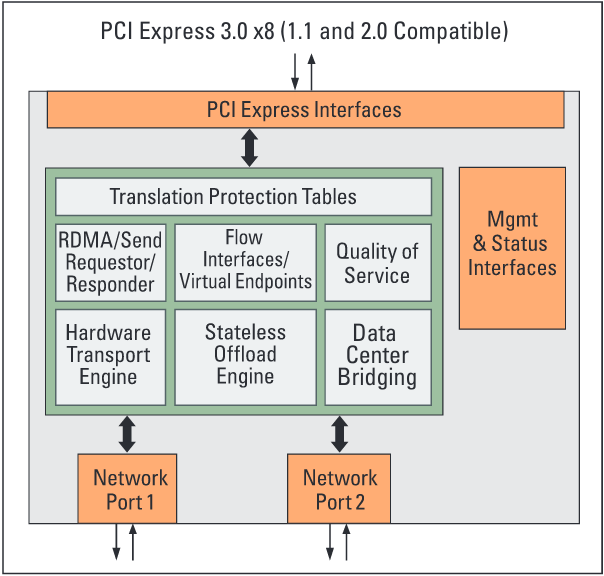
\includegraphics[width=7.5cm,keepaspectratio]{fig/mlx-block-diagram.png}
	\caption{Mellanox ConnectX-3 EN block diagram (source:~\cite{mellanox-silicon})}
	\label{fig:setup-mlx-block-diagram}
	\bigskip
\end{figure}

The Mellanox NIC requires PCI-Express 3.0 x8 slot to take full advantage of its speed.
Brno University of Technology provided a server with
the Supermicro X10DRU-i+ motherboard, which
features PCI-Express 3.0 slots compatible with the Mellanox Connect-X 3 EN adapter~\cite{supermicro-board}.
The server is further equipped with two Intel Xeon E5-2660 v3 processors at 2200MHz with 10 physical cores per CPU
and 20 logical cores per CPU when Hyper-Threading is enabled.
Each CPU has 20MB shared L3 cache and PCI Express 3.0 support with up to 40 lanes.
The processor features Direct Data I/O technology (also known as Direct Cache Access),
which optimises cache access for networking purposes by putting the ingress packtes directly to the CPU cache~\cite{intel-xeon-cpu}.

There are various software frameworks for high-speed packet generation,
such as pktgen\footnote{\url{https://www.kernel.org/doc/Documentation/networking/pktgen.txt}}
or Netmap\footnote{\url{http://info.iet.unipi.it/~luigi/netmap/}}.
Pktgen is an upstream component of the Linux kernel, but
at the time of writing it is not capable of generating even full 10~GbE frame rate~\cite{netmap}.
However, it can be combined with other frameworks for fast packet processing, such as
Intel's Data Plane Development Kit\footnote{\url{http://dpdk.org/}}.
Netmap provides patches to the Linux kernel.
Netmap claims to generate 14.88~million frames per second, which is a full frame rate of 10~Gigabit Ethernet~\cite{netmap}.
However, Netmap was not tested against 40~GbE full frame rate of 59.5~million frames per second,
as calculated in section~\ref{sec:40gbe-frame-rates}.
Although both the frameworks seem promising, their benchmarking and description
are outside the scope of this thesis.
Moreover, to perform the measurements of a software-based packet generator,
another GNU/Linux server and a 40~GbE NIC is needed.

Another solution is to use a hardware-based packet generator such as Spirent~\cite{spirent}.
With kind permission of CESNET, the Czech national research and education network operator,
the Spirent SPT-3U equipped with a combined 100Gb / 2x40Gb Ethernet module was used to perform the measurements.
The Spirent packet generator supports generation of custom Layer 2-7 traffic, custom frame length and various
predefined traffic patterns with variable frame length called Internet Mix (iMix).
These patterns represent a typical distribution of frame lengths found in the Internet traffic
and they can be further customised.
Spirent SPT-3U further supports configuration of custom frame rates and bandwidth use~\cite{spirent}.
